\documentclass[conference]{IEEEtran}
\IEEEoverridecommandlockouts
% The preceding line is only needed to identify funding in the first footnote. If that is unneeded, please comment it out.
\usepackage{cite}
\usepackage{amsmath,amssymb,amsfonts}
\usepackage{systeme}
\usepackage{algorithmic}
\usepackage{graphicx}
\usepackage{textcomp}
\usepackage{xcolor}
\usepackage{flushend}
\usepackage{float}
\usepackage{lmodern}
\usepackage[]{algorithm2e}
\usepackage{times}
\usepackage[bookmarks=false]{hyperref}
\usepackage{pgfplots}
\usepackage{booktabs}
\usepackage{subfigure}
\usepackage[a4paper, left=0.51in, right=0.51in, top=0.75in, bottom=1.69in]{geometry}
\usepackage{listings}
\lstset{
	% --- Estilo da Fonte ---
	basicstyle=\ttfamily\small,   % Fonte: monoespaçada e pequena.
	% --- Estilos de Sintaxe (COM CORES) ---
	keywordstyle=\color{blue}\bfseries, % Palavras-chave: azul e negrito.
	commentstyle=\color[rgb]{0.1,0.5,0.1}, % Comentários: verde escuro.
	stringstyle=\color{red},            % Strings ("texto"): vermelho.
	% --- Formatação ---
	showstringspaces=false,       % Não marca espaços em strings.
	breaklines=true,              % Quebra linhas longas.
	frame=single,                 % Borda simples (caixa).
	numbers=left,                 % Números à esquerda.
	% --- Estilo dos Números (NOVO) ---
	numberstyle=\tiny, % Tamanho reduzido e cor cinza
	xleftmargin=20pt,       % Empurra todo o bloco de código para a direita, afastando-o da coluna vizinha
	framexleftmargin=15pt,
}

\newcommand{\sandro}[1]{{\color{red}[#1]}}		
\newcommand{\lucas}[1]{{\color{blue}[#1]}}


\def\BibTeX{{\rm B\kern-.05em{\sc i\kern-.025em b}\kern-.08em
    T\kern-.1667em\lower.7ex\hbox{E}\kern-.125emX}}
    
    \IEEEoverridecommandlockouts
\IEEEpubid{%
\makebox[\columnwidth]{%
978-1-7281-7539-3/20/\$31.00~\copyright{}2020 IEEE\hfill%
} \hspace{\columnsep}\makebox[\columnwidth]{ }%
}
\begin{document}

\title{\noindent 
	\begin{minipage}[c]{0.1\textwidth}
		
\includegraphics[width=2.2cm]{Imagens/logo} 
	\end{minipage}
	\begin{minipage}[c]{0.8\textwidth}
		\centering 
		\fontsize{12}{14}\selectfont
		Universidade Federal de Itajubá - UNIFEI - Campus Itabira \\
		Curso de Engenharia da Computação - ECO \\
		Computação Gráfica e Processamento Digital de Imagens  \\
		Prof. Dr. André Ribeiro de Brito
	\end{minipage}
	\vspace{1cm} \\ 
	\LARGE \textbf{Avião em Movimento}
}

\author{\IEEEauthorblockN{Fabrício Rickelmer Souza Duarte }
	\IEEEauthorblockA{Instituto de Ciências Tecnológicas, Universidade Federal de Itajubá, Itabira, Minas Gerais, Brazil}
	\textit{d2023012884@unifei.edu.br} \\
	\text{R.A: 2023012884}}
	
\maketitle

\begin{abstract}
	Esse artigo tem como fundamento a implementação de um algoritmo de computação gráfica de um modelo 3d de um avião em movimento, demonstrando as funções básicas do OpenGL, para o estudo da matéria de Computação Gráfica e Processamento Digital de Imagens ministrada na UNIFEI pelo professor e doutor André Ribeiro de Brito. O objeto do avião pode ser visualizado de diversas formas com o movimento da câmera, ter a movimentação acelerada e reduzida, aumentado de tamanho e ter o movimento pausado através da implementação do código.
\end{abstract}
\renewcommand\IEEEkeywordsname{Keywords}
\begin{IEEEkeywords}
	Computação, gráfica, modelagem, OpenGL, avião.
\end{IEEEkeywords}

%----------------------------------------------------

\section{Introdução}

O trabalho tem como objetivo de colocar em prática os conceitos aprendidos em sala de aula na matéria de computação gráfica e processamento digital de imagens sobre o uso da biblioteca gráfica openGL para a criação de objetos através de código.

Foi utilizado como IDE o vscode em conjunto com o openGL no sistema operacional do windows para a criação e modelagem de uma cena de um avião voando ao lado de nuvens, com possibilidade de interações com transformações geométricas e movimentação de camera, através do teclado. As interações possibilitam o movimento de câmera, mudança do foco, reset para câmera original, pausa, velocidade de movimento, tamanho e fechamento da janela da cena.

O vscode foi usado para criação do código com o openGL que é a API, responsável pelo intermédio do código com o hardware, sendo aberta e com funções matemáticas que são transcrevidas em imagens na tela.

\begin{figure}[H]
	\centering
	
	\caption{Demonstração da Cena do Avião}
	\vspace{0.2cm}
	
	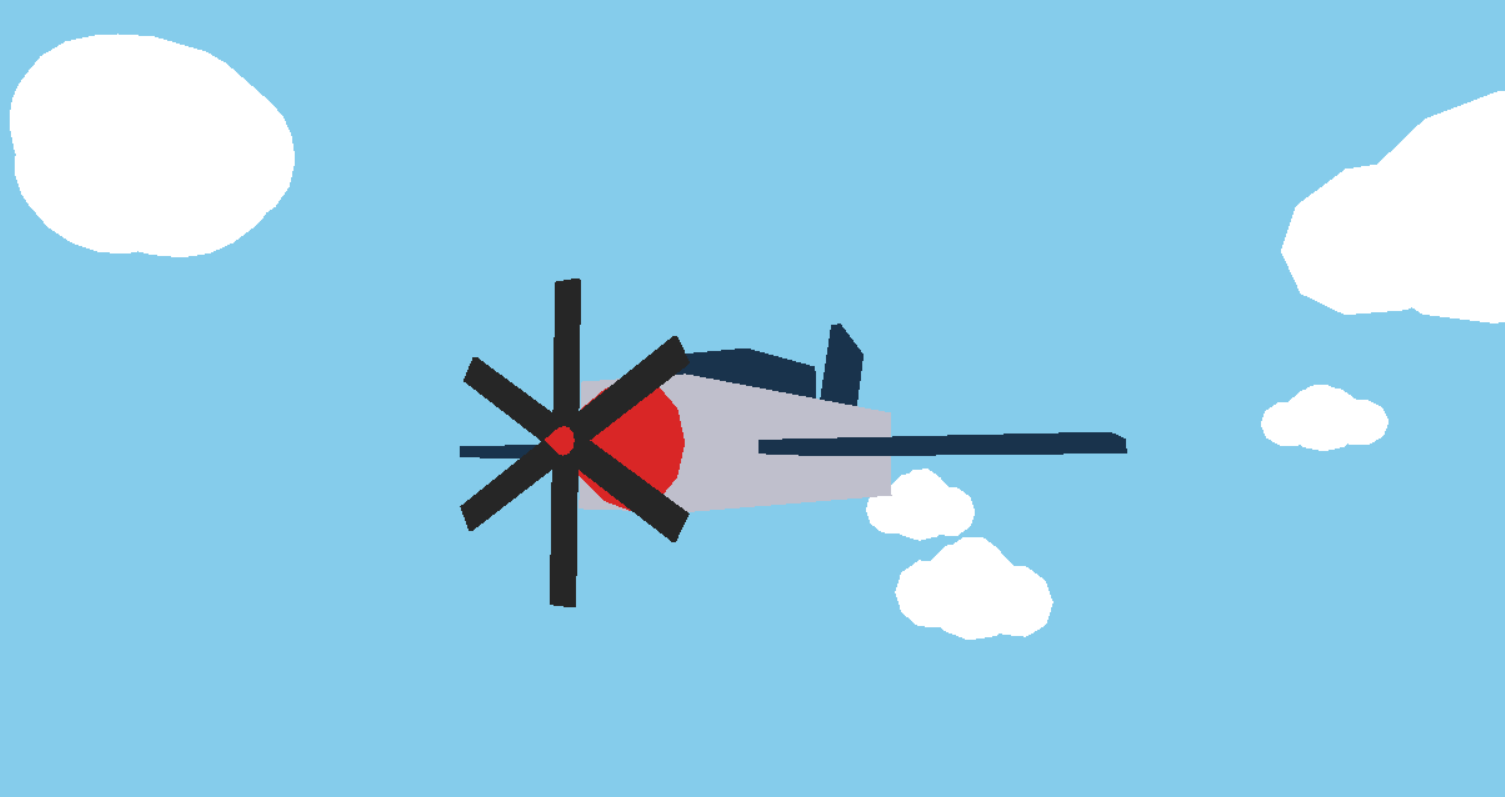
\includegraphics[width=\linewidth]{Imagens/aviao (3).png}
	
	{\footnotesize Fonte: Autoria Própria (2026).}
\end{figure}

A cena utiliza modelos primitivos, para a criação dos objetos, e transformações, para realizar o movimento e mudanças do objeto, demonstrando os conceitos dados em sala.

\section{Desenvolvimento}

O desenvolvimento do projeto teve como base os exemplos dados em sala de aula pelo professor, com o carrinho se movimentando e mudando conforme as definições eram ensinadas, códigos passados via Sistema Integrado de Gestão de Atividades Acadêmicas (SIGAA) e slides dados em sala. Foi utilizada uma ferramenta Large Language Model (LLM) chamada gemini para orientação na produção do código, definições de conceitos de computação gráfica e busca por referências.

\subsection{Resultados}

A realização do trabalho permitiu colocar em prática e aprender sobre como a computação gráfica é feita e foi possível com ela entender mais sobre modelagem e assuntos relacionados.

Ao final as principais funções criadas e utilizadas no desenvolvimento do código foram init(), para configurar o estado base do OpenGL antes para poder renderizar os modelos; desenhaNuvem(), para desenhar os objetos das nuvens; desenhaCaixaTexturizada(), para colocar as textura; desenhaAviao(), para inserir o avião na cena; display(), renderiza os frames da cena; atualizaCena(), faz o movimento do avião; teclado(), realiza a modificação do comportamento conforme a tecla pressionada. 

\begin{figure}[H]
	\centering
	
	\caption{Movimentação de Câmera - Visão Inferior}
	\vspace{0.2cm}
	
	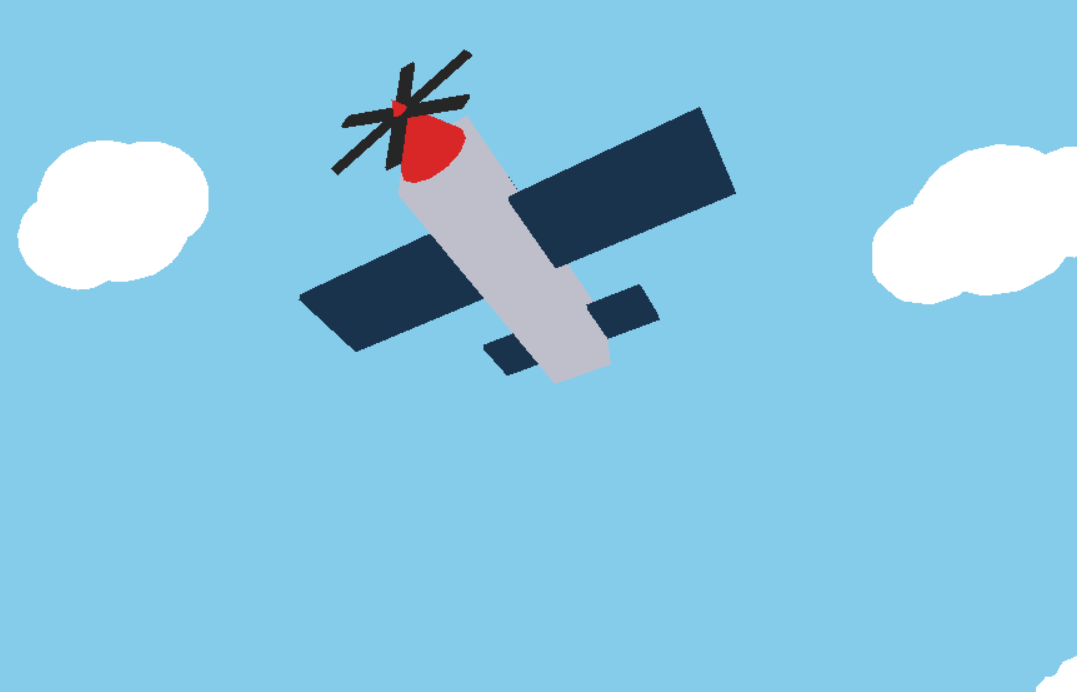
\includegraphics[width=\linewidth]{Imagens/aviao (2).png}
	
	{\footnotesize Fonte: Autoria Própria (2026).}
\end{figure}

\begin{figure}[H]
	\centering
	
	\caption{Movimentação de Câmera - Visão Superior}
	\vspace{0.2cm}
	
	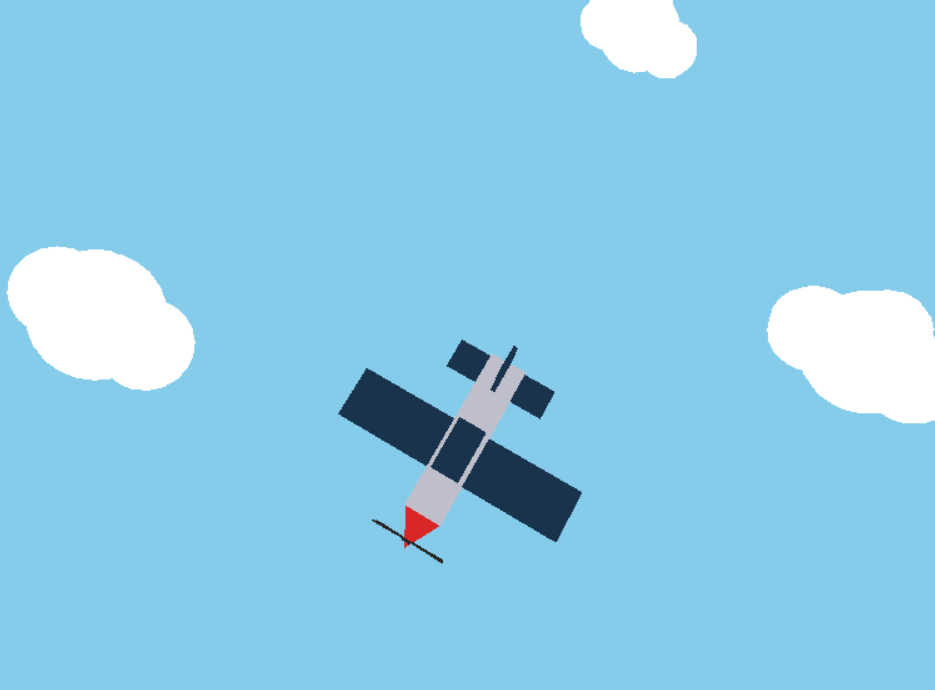
\includegraphics[width=\linewidth]{Imagens/aviao (1).png}
	
	{\footnotesize Fonte: Autoria Própria (2026).}
\end{figure}

\subsection{Discussão}

Houveram dificuldades para a instalação da biblioteca por não ter tido contato anteriormente e implementação de certas funções como a movimentação da câmera.

\section{Considerações Finais}

A implementação cumpriu com as exigências propostas para a conclusão do trabalho de forma objetiva, porém com o tempo poderia ser mais elaborada e desenvolvida, com maior quantidade de modelos e movimentos com mais opções de interação.

\begin{thebibliography}{9}
	
	\bibitem{redbook}
	SHREINER, D.; SELLERS, G.; KESSENICH, J.; LICEA-KANE, B. \textbf{OpenGL Programming Guide: The Official Guide to Learning OpenGL}. 8. ed. Addison-Wesley Professional, 2013.
	
	\bibitem{angel}
	ANGEL, E.; SHREINER, D. \textbf{Interactive Computer Graphics: A Top-Down Approach with Shader-Based OpenGL}. 6. ed. Pearson Education, 2011.
	
	\bibitem{opengl_ref}
	Khronos Group. \textbf{OpenGL 2.1 Reference Pages}. 2026. Disponível em: \url{https://www.khronos.org/registry/OpenGL-Refpages/gl2.1/}. Acesso em: 29 set. 2026.
	
	\bibitem{freeglut}
	FreeGLUT Contributors. \textbf{The FreeGLUT Project API Documentation}. 2026. Disponível em: \url{https://freeglut.sourceforge.net/docs/api.php}. Acesso em: 29 set. 2026.
	
	\bibitem{trabalhocg}
	Disciplina de Computação Gráfica e Processamento Digital de Imagens. \textbf{Trabalho Prático - OpenGL}. Material de avaliação disponibilizado via SIGAA. Universidade Federal de Itajubá (UNIFEI) - Campus Itabira. 2026.
	
	\bibitem{github_repo}
	RICKELMER, F. \textbf{TrabalhoComputacaoGrafica}: Código-fonte do projeto de animação e modelagem 3D em OpenGL. GitHub, 2026. Disponível em: \url{https://github.com/FabricioRickelmer/TrabalhoComputacaoGrafica}. Acesso em: 29 set. 2026.
	
\end{thebibliography}
\end{document}